\documentclass[letterpaper,10pt,conference]{ieeeconf}
\IEEEoverridecommandlockouts
\overrideIEEEmargins
\usepackage[T1]{fontenc}
\usepackage[utf8]{inputenc}
\usepackage{amsmath,amssymb}
\usepackage{booktabs,array,tabularx}
\usepackage{graphicx}
\usepackage{url}
\usepackage[hidelinks]{hyperref}
\urlstyle{same}
\newcolumntype{Y}{>{\raggedright\arraybackslash}X}

\title{\LARGE\bf Compact Visuotactile World Models for Lifting:\protect\\
Prediction, Reward Alignment, and Force Constraints}
\author{Qinzhen Ma$^{1}$ and Sida Peng$^{2}$%
\thanks{$^{1}$Qinzhen Ma is with Rice University.
Corresponding author: {\tt\small qm18@rice.edu}.}%
\thanks{$^{2}$Sida Peng is with Zhejiang University.}}
\hypersetup{
pdftitle={Compact Visuotactile World Models for Lifting: Prediction, Reward Alignment, and Force Constraints},
pdfauthor={Qinzhen Ma and Sida Peng},
pdfsubject={Robotics; visuotactile prediction and model-based control},
pdfkeywords={visuotactile world models, tactile sensing, model-based reinforcement learning, force constraints}}

\begin{document}
\maketitle
\thispagestyle{plain}
\pagestyle{plain}

\begin{abstract}
Accurate contact prediction is useful for robotic manipulation only if it supports effective decisions. We investigate this connection using a compact, randomly initialized visuotactile world model, trajectory-level uncertainty calibration, and behavior-initialized actor--critic learning in imagination. On 160 MuJoCo Lift episodes, adding touch reduces endpoint-force prediction error from 1.058 to 0.228 N and interval-peak error from 2.724 to 0.523 N across three training seeds. However, tactile persistence achieves lower errors of 0.095 and 0.498 N, respectively. Two exploratory control rounds comprise 680 executions on 40 independent test initial conditions. A matched reward revision on fresh test environments increases in-distribution 10 cm lifting success from 20.0\% to 93.3\%, while success within an 8 N per-finger budget reaches only 33.3\%, compared with 70.0\% for force feedback. Calibration margins reduce force violations at the cost of task completion. In a separate study of public GelSight recordings, a force regressor achieves 0.04234 N error, but frame-level calibration covers only 15.80\% of complete trajectories; trajectory-level calibration raises this to 87.36\% at nominal 90\% coverage. Together, these findings distinguish improvements in sensing and task reward from improvements in force-constrained control. The evidence is limited to public sensing records and simulator execution, without a demonstrated transfer between them.
\end{abstract}

\section{Introduction}

Contact-rich manipulation couples perception, prediction, and control. Vision
observes object geometry and motion, while touch supplies local evidence about
contact forces. Compact models that combine these signals are attractive for
short-horizon control, but a reduction in prediction error need not yield a
better policy. Slowly varying contacts may be predicted well by persistence;
a learned policy may optimize a reward that differs from the task criterion;
and infrequent force peaks may dominate a constraint despite a small average
forecast error.

We study these three issues in grasp closure and lifting. Our question is
whether the benefits of tactile observations survive the successive steps
from force prediction to trajectory-level reliability and executed control.
The distinction matters physically: before an object leaves its support,
the force borne by the gripper does not determine object mass, and sticking
contact does not uniquely identify friction. We therefore evaluate forecasts
and explicit force budgets rather than infer unobserved material properties
or damage thresholds.

The study has two complementary experimental branches. Public optical tactile
recordings with independently measured forces test perception and the effect
of calibrating entire contact trajectories. A modified robosuite Lift task
tests action-conditioned forecasting and policies trained inside a frozen
world model. Its tactile inputs are simulator contact-force aggregates. These
branches share a question about prediction reliability, but do not constitute
a sensor-transfer or sim-to-real pipeline.

Our contributions are three empirical findings. First, a 652,157-parameter
model benefits from aligned touch relative to vision-only input, yet loses to
persistence on several force metrics. Second, trajectory calibration exposes
tail errors that are obscured by average accuracy and frame coverage. Third,
a matched reward revision improves executed lifting on fresh environments,
while remaining inferior to force feedback on force-budgeted success.
Together, the matched comparisons identify a correctable reward mismatch and
the separate dynamics and constraint limitations that remain after it is
corrected. The accompanying code and tabulated results document these
comparisons and their evaluation units.

\begin{figure*}[t]
\centering
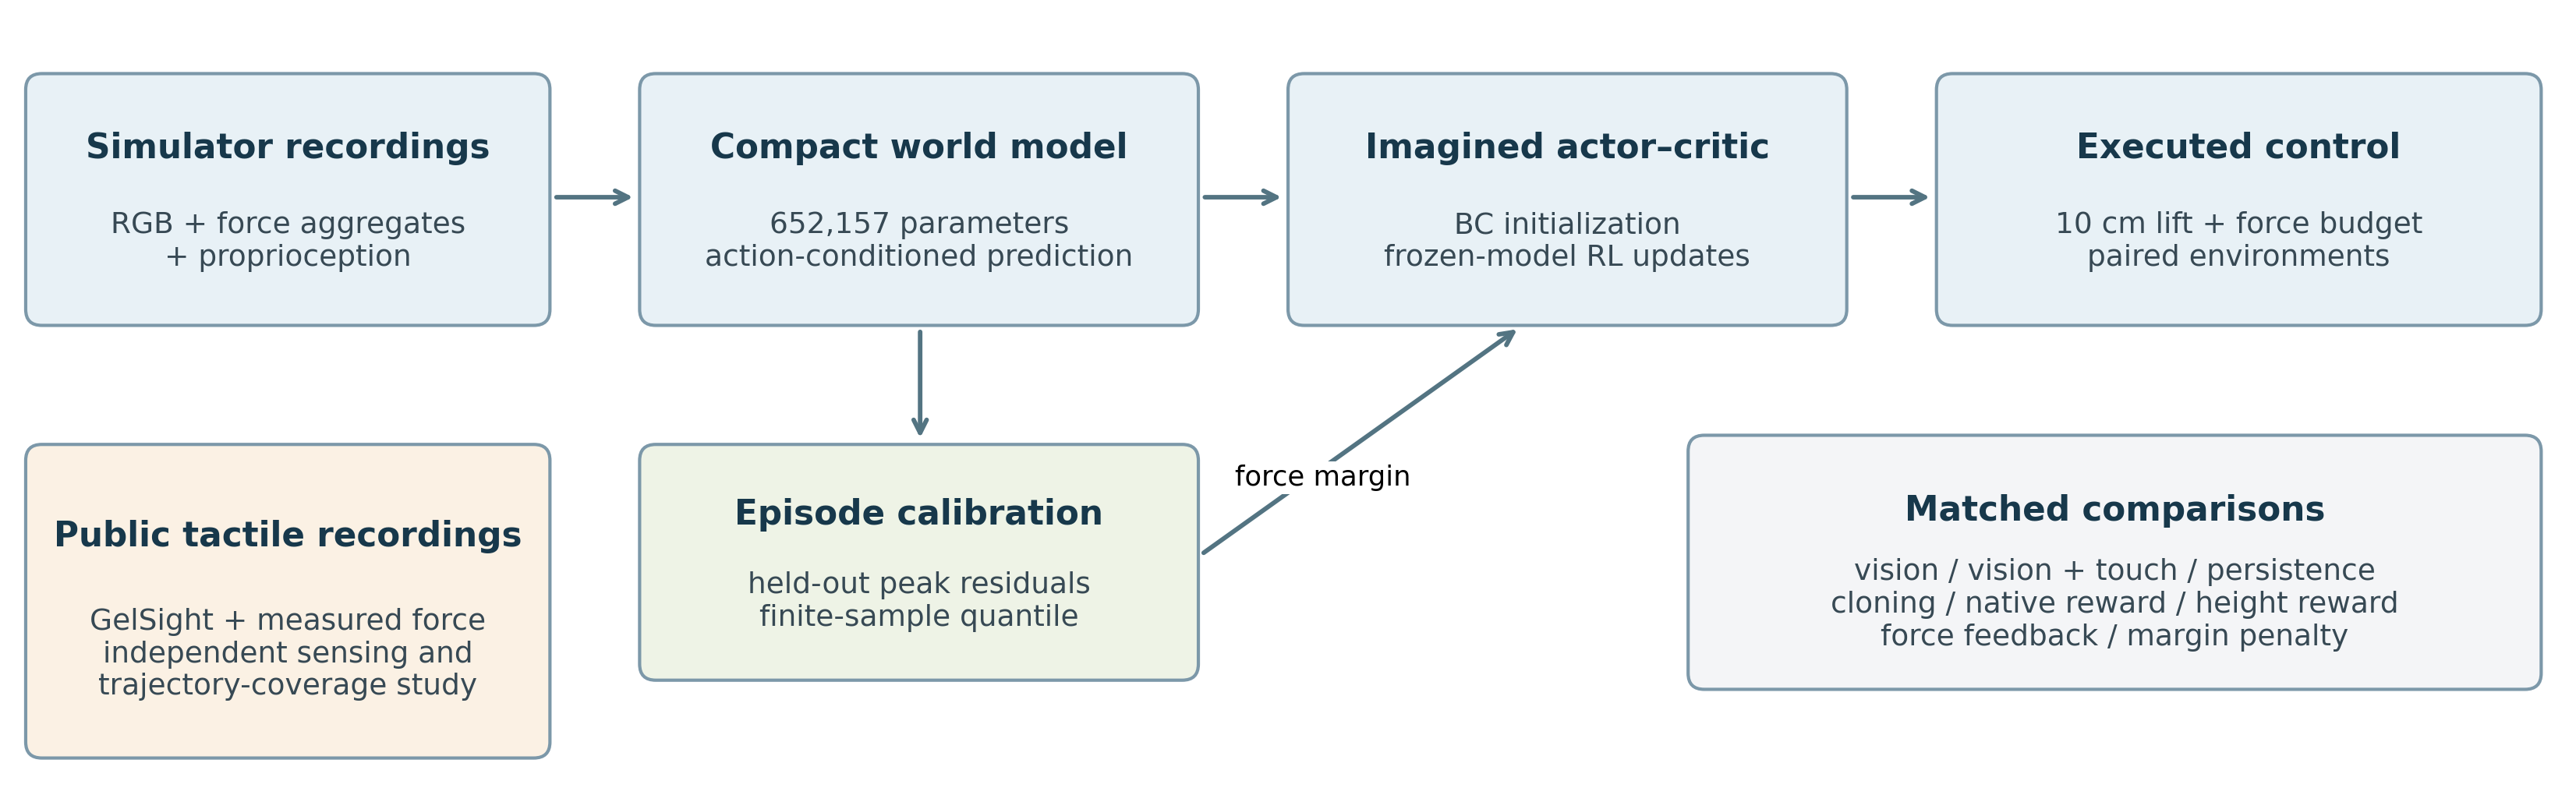
\includegraphics[width=\textwidth]{architecture.png}
\caption{Experimental design. The simulator branch uses contact-force
aggregates; the public-data branch uses optical tactile images and supplies a
separate sensing study. The actor learns inside a frozen world model, and its
performance is measured by executing actions in MuJoCo.}
\label{fig:architecture}
\end{figure*}

\section{Related Work}

Sparsh provides tactile representations and TacBench force-estimation
data~\cite{sparsh}. FeelAnyForce studies contact-force estimation and transfer
across optical tactile sensors~\cite{feelanyforce}. These works motivate using
actual force measurements to evaluate perception, rather than treating a
derived slip label as independent evidence.

Visuotactile world modeling is already established. VT-WM combines vision,
touch, action-conditioned prediction, and planning~\cite{vtwm}. FeelWorld
explicitly predicts contact, force-related representations, and
slip~\cite{feelworld}. OmniVTA combines short-horizon tactile prediction with
reactive feedback~\cite{omnivta}. Consequently, modality fusion or predicting
contact is not our novelty claim. Our focus is the connection between compact
contact forecasts, trajectory-level error accounting, and the usefulness of
resulting decisions.

TD-MPC2 supplies scalable latent dynamics and planning components~\cite{tdmpc2}.
We adapt its open-source convolutional, MLP, and SimNorm building blocks, rather
than reproducing its complete learning algorithm. Conformal prediction provides
finite-sample calibration under exchangeability~\cite{conformal}, while
Conformal Decision Theory directly addresses decisions made from imperfect
predictions~\cite{cdt}. Our task-specific residuals use standard split-conformal calibration with a
fixed predictor. We do not implement the decision-risk control
procedure of Conformal Decision Theory or introduce a new coverage theorem.

\section{Method}

\subsection{Compact action-conditioned model}

The observation history contains three $64\times64$ external RGB frames, three
tactile observations, and three proprioceptive observations. In simulation,
touch comprises a normal force and two signed tangential components for each
finger. The tangent basis is fixed using projected gravity-up and its cross
direction. These signals are simulated contact-force aggregates, not optical
tactile images. Proprioception contains end-effector position, orientation, and
finger positions.

A four-layer convolutional encoder produces a 256-dimensional visual feature.
Separate MLPs produce 64-dimensional tactile and 32-dimensional proprioceptive
features. Their concatenation is projected to a 128-dimensional SimNorm latent:
\begin{equation}
\begin{aligned}
z_t &= e_\theta(o_{t-2:t}),\\
\widehat z_{t+k+1} &= d_\theta(\widehat z_{t+k},a_{t+k}).
\end{aligned}
\label{eq:dynamics}
\end{equation}
The transition network has two 384-unit hidden layers. Heads predict endpoint
force, relative object height, table support, finger contact, native task
reward, and a $16\times16$ RGB auxiliary target. A dedicated pair of outputs
predicts each finger's maximum normal force over all physics substeps between
observations; endpoint force alone could miss transient peaks. The
implementation has 652,157 trainable parameters and is initialized randomly,
without pretrained weights. Object state, interval peaks,
and contact labels supervise training but never enter the encoder or actor as
privileged inputs.

Training unrolls five predicted transitions. Losses combine normalized Huber
regression for endpoint force, interval-peak force, height, and reward;
binary contact/support losses;
low-resolution image error; and consistency with a stop-gradient
exponential-moving-average encoder. Future observations are used only as
targets. Normalization statistics use training episodes exclusively. Validation
selects the checkpoint. Vision-only and visuotactile variants have identical
parameter counts; the vision-only variant masks normalized tactile inputs to
zero.

\subsection{Contact-envelope calibration}

For the independent public-force experiment, let $F=(F_x,F_y,F_n)$, with
compression-positive normal force, and define
\begin{equation}
g_\mu(F)=\sqrt{F_x^2+F_y^2}-\mu F_n.
\label{eq:contact-function}
\end{equation}
The parameters $\mu\in[0.3,0.8]$ and normal-force ceilings are specified
analysis conditions. They are neither identified friction coefficients nor
measured damage thresholds. A one-sided joint residual is
\begin{equation}
s_{it}=\max\left\{
\begin{aligned}
&g_{0.3}(F_{it})-g_{0.3}(\widehat F_{it}),\\
&g_{0.8}(F_{it})-g_{0.8}(\widehat F_{it}),\\
&F_{n,it}-\widehat F_{n,it}
\end{aligned}
\right\}.
\label{eq:residual}
\end{equation}
The residual difference is affine in $\mu$, so its endpoint maximum bounds
the full interval. We compare pooling frame scores with calibrating
$S_i=\max_t s_{it}$ over complete contact trajectories. For $n$ calibration
units, the corrected quantile uses rank $\lceil(n+1)(1-\alpha)\rceil$;
negative quantiles are clipped to zero. Insufficient calibration units imply
an infinite bound.

The resulting upper bounds are $g_\mu(\widehat F)+q$ and $\widehat F_n+q$.
A frame passes the analysis envelope only if both bounds satisfy their
specified limits. A coordinate-box baseline instead calibrates the maximum
absolute error over coordinates and time, then propagates its box through the
contact functions.

Conditional on a fixed predictor and exchangeable calibration/test trajectories,
the trajectory construction supplies marginal simultaneous coverage. It does
not guarantee coverage under shape shift, an adaptively selected control
distribution, or a new closed-loop policy. Nor does marginal coverage bound
error conditional on acceptance. We report acceptance and conditional
violations separately, and leave conditional error undefined when nothing is
accepted.

For the simulator world model, calibration instead uses the positive underprediction residual of per-finger interval peaks and the absolute height residual. Each score is maximized over the episode's evaluated windows and all five future steps; the force score also maximizes over fingers. We allocate error probability $\alpha/2$ to each of the two quantities and compute separate corrected quantiles. The peak at state $t+1$ summarizes the physics substeps produced by action $a_t$, so evaluation never substitutes the endpoint contact reading for the interval target. These bounds concern forecasts along recorded actions, not all counterfactual actions.

\subsection{Imagined policy learning}
\label{sec:policy}

The policy-learning stage freezes the world model and initializes a
two-output actor by behavior cloning. Its outputs control vertical motion and
continuous gripper opening/closing after a common scripted approach. Each
output is mapped into the corresponding training-action range; this limits
action extrapolation but does not guarantee state-distribution support.

Starting from encoded training observations, the actor rolls the model forward
for five steps. It maximizes discounted predicted task reward, penalized by
predicted interval-peak normal-force excess, action magnitude, and deviation
from the frozen behavior prior. A value network regresses detached imagined
return targets. An EMA target critic supplies a terminal bootstrap while
retaining gradients through the terminal latent for actor learning. Simulator
rewards and object state are never queried during imagined updates.

For two-dimensional action $u_k$, predicted per-finger peak $\widehat p_{kj}$,
force budget $B=8$ N, and margin $q$, the imagined stage reward is
\begin{equation}
\begin{aligned}
\widetilde r_k={}&\widehat r_k-\frac12\sum_{j=1}^2
\left(\frac{[\max(0,\widehat p_{kj})+q-B]_+}{B}\right)^2\\
&-\frac{0.005}{2}\|u_k\|_2^2.
\end{aligned}
\label{eq:imagined-reward}
\end{equation}
We use $q=0$ for ordinary imagined RL and the fixed calibration allowance
for the margin variant. Returns obey $G_k=\widetilde r_k+0.95G_{k+1}$;
the terminal critic bootstrap is zero at the intervention boundary. The actor
minimizes $-G_0$ plus twice the mean squared action deviation from the frozen
behavior prior. Training uses 3,520 encoded starts from training episodes,
1,000 behavior-cloning updates, and 1,500 imagined updates, with batch size
256. Adam learning rates are $2\times10^{-4}$ for the actor and
$3\times10^{-4}$ for the critic. There is no online data collection or
world-model retraining during these updates.

This actor--critic objective differs from the official TD-MPC2 algorithm.
We evaluate the learned policies independently in the simulator because
optimization can exploit model errors and change the state distribution on
which recording-based calibration was obtained.

\section{Public Tactile-Force Study}

\subsection{Data and protocol}

We use the public GelSight force dataset from TacBench, revision
\texttt{136d\allowbreak{}b554\allowbreak{}85b6\allowbreak{}5016\allowbreak{}05b1\allowbreak{}d264\allowbreak{}8ce0\allowbreak{}fe44\allowbreak{}740e\allowbreak{}302e}~\cite{sparsh}. GelSight
Mini images are paired with ATI Nano17 force measurements. The converted data
contain 102,628 paired frames from 1,513 loading/shear trajectories. This
dataset contains neither external scene RGB nor the action/reward sequences
needed for our world model.

Sphere batches 1--5 are partitioned by entire trajectory: training 453
trajectories/33,982 frames, validation 75/5,983, calibration 114/8,343, and
testing 116/9,003. Sphere batch 6 and all flat/sharp trajectories are held out.
No adjacent frames from the same trajectory cross partitions. Flat/sharp
records contain five unmatched trailing image indices; only paired entries
are retained, and these tests remain exploratory. A fixed $-5/0/+5$-frame
sensitivity analysis uses matched central frames without choosing an offset
from test performance.

The regressor is a 361,091-parameter CNN, trained for at most 30 epochs with
AdamW and validation-based selection. Three seeds share the same split. Force
statistics use only training labels. Slip labels supplied by the dataset are
derived through a friction-cone procedure and are excluded from independent
slip evaluation.

\subsection{Force prediction and distribution shift}

\begin{table}[t]
\caption{Force prediction on held-out public tactile records.}
\label{tab:force}
\centering
\small
\setlength{\tabcolsep}{3pt}
\begin{tabularx}{\columnwidth}{@{}Yrrr@{}}
\toprule
Test distribution & \shortstack{Trajectories/\\frames}
 & \shortstack{CNN\\MAE, N}
 & \shortstack{Training-mean\\baseline, N}\\
\midrule
Sphere, held-out trajectories & 116 / 9,003 & 0.04234 & 0.11870\\
Sphere, held-out batch 6 & 153 / 11,364 & 0.03915 & 0.11322\\
Flat, exploratory shape shift & 298 / 13,045 & 0.32685 & 0.13783\\
Sharp, exploratory shape shift & 304 / 20,908 & 0.41304 & 0.12432\\
\bottomrule
\end{tabularx}
\end{table}

Across seeds, sphere MAE is $0.04234\pm0.00306$ N and batch-6 MAE is
$0.03915\pm0.00351$ N; $\pm$ denotes training-seed standard deviation. A
grouped bootstrap yields a 95\% interval of [0.03823, 0.04675] N for sphere
MAE. The regressor performs worse than the constant baseline on the held-out
shapes, indicating poor cross-shape generalization in this protocol. Batch identifiers alone
do not establish cross-day or cross-sensor transfer.

\subsection{Frame reliability does not imply trajectory reliability}

Table~\ref{tab:coverage} reports joint contact-function coverage at nominal $\alpha=0.10$.

\begin{table}[t]
\caption{Joint contact-function coverage at nominal $\alpha=0.10$.
Allowances average over frames, the three tested $\mu$ values, and training
seeds; the propagated box allowance is not its coordinate radius.}
\label{tab:coverage}
\centering
\small
\setlength{\tabcolsep}{3pt}
\begin{tabularx}{\columnwidth}{@{}Yrrr@{}}
\toprule
Calibration & \shortstack{Frame\\coverage}
 & \shortstack{Trajectory\\coverage}
 & \shortstack{Mean contact-bound\\allowance, N}\\
\midrule
Uncalibrated prediction & 34.30\% & 0.00\% & 0\\
Frame, direct functions & 89.62\% & 15.80\% & 0.1096\\
Trajectory, propagated coordinate box & 99.87\% & 99.14\% & 0.6878\\
Trajectory, direct functions & 99.24\% & 87.36\% & 0.3338\\
\bottomrule
\end{tabularx}
\end{table}

Direct trajectory calibration narrows the allowance relative to box
propagation, but its observed trajectory coverage is lower and does not reach
the nominal 90\%. The grouped-bootstrap 95\% interval is [81.90\%, 92.24\%].
The narrower bounds therefore trade coverage for a smaller allowance in this sample.

For the illustrative envelope $\mu=0.8,F_n\leq2$ N, box propagation accepts
no frames. Direct trajectory calibration accepts 18.84\%, with 0.192\%
conditional proxy-constraint violations. This is offline classification of
measured forces, not success after executing a robot action. All tested
coefficients, ceilings, and zero-acceptance cases are retained in the ancillary
metric tables.

\section{Simulator World-Model and Interaction Study}

\subsection{Data and evaluation protocol}

We execute a modified robosuite 1.5.1 Panda Lift task~\cite{robosuite} in MuJoCo 3.3.7~\cite{mujoco}, with continuous gripper-rate control. The dataset contains 160 episodes of 150 actions at 20 Hz, with 25 physics substeps per action. Entire episodes are split into 80 training, 16 validation, 24 calibration, 20 in-distribution (ID) test, and 20 out-of-distribution (OOD) test episodes. The cube geometry is fixed. ID mass is sampled from \{0.06, 0.12, 0.25, 0.40\} kg and sliding friction from \{0.35, 0.60, 0.90\}; OOD uses \{0.65, 0.90\} kg and \{0.12, 0.22\}. Both finger and object friction are changed. This joint shift does not isolate either physical factor. Per-finger actuator limits vary over 3, 6, 12, and 20 N; these differ from the contact-force budget and can also limit feasibility within the ID domain.

Three seeds train each modality variant for 25 epochs, using training-window stride three and a five-transition horizon. Evaluation uses stride five, yielding 600 windows from 20 episodes in each test split. All reported forecasts follow recorded actions and are compared against actual simulator states. The model adapts TD-MPC2 building blocks with random initialization; it is neither a pretrained model nor a reproduction of the full TD-MPC2 algorithm.

\subsection{Forecasts and the persistence counterexample}

\begin{table}[t]
\caption{World-model forecast MAE, averaged over horizons one through five.
Values are mean $\pm$ sample standard deviation across three training seeds.}
\label{tab:world-model}
\centering
\small
\setlength{\tabcolsep}{3pt}
\begin{tabularx}{\columnwidth}{@{}Yccc@{}}
\toprule
Split / input & \shortstack{Endpoint\\N} & \shortstack{Interval peak\\N}
 & \shortstack{Height\\mm}\\
\midrule
ID / vision & $1.058\pm0.062$ & $2.724\pm0.287$ & $3.946\pm0.561$\\
ID / V+T & $0.228\pm0.029$ & $0.523\pm0.051$ & $2.822\pm0.336$\\
OOD / vision & $0.768\pm0.044$ & $1.918\pm0.106$ & $2.637\pm0.425$\\
OOD / V+T & $0.373\pm0.024$ & $0.849\pm0.100$ & $2.321\pm0.405$\\
\bottomrule
\end{tabularx}
\end{table}

\begin{table*}[t]
\caption{Initial-round executed control on the same 20 new environments: ten ID and ten OOD.
Learned methods average three fixed policies; the sample is not 60 independent
environments. All OOD strict and joint successes are zero.}
\label{tab:control}
\centering
\small
\setlength{\tabcolsep}{5pt}
\begin{tabularx}{\textwidth}{@{}Yrrrrr@{}}
\toprule
Controller & \shortstack{Strict lift\\\%} & \shortstack{Lift within 8 N\\\%}
 & \shortstack{Exceeds 8 N\\\%} & \shortstack{Mean episode peak\\N} & Native return\\
\midrule
Script & 35.0 & 10.0 & 55.0 & 10.269 & 56.646\\
Force feedback & 40.0 & 25.0 & 30.0 & 7.175 & 59.815\\
Vision BC & 15.0 & 5.0 & 48.3 & 8.564 & 48.517\\
Vision RL & 6.7 & 5.0 & 83.3 & 12.452 & 41.089\\
Vision + touch BC & 15.0 & 5.0 & 56.7 & 9.955 & 55.943\\
Vision + touch RL & 6.7 & 3.3 & 61.7 & 9.478 & 61.365\\
Vision + touch margin RL & 5.0 & 5.0 & 8.3 & 3.210 & 51.164\\
\bottomrule
\end{tabularx}
\end{table*}

Table~\ref{tab:world-model} averages horizons one through five and reports the mean $\pm$ sample standard deviation over three training seeds. V+T denotes vision and touch. Endpoint force averages six signed/contact components; peak force averages two normal-force maxima. These are distinct targets. Touch reduces both errors relative to vision in each split.

Contact occurs at 1,441/3,000 ID forecast points and 717/3,000 OOD points. Restricting endpoint error to actual contact raises vision MAE to 2.087/2.548 N for ID/OOD, and visuotactile MAE to 0.409/1.131 N. Thus, the lower all-phase vision error on OOD reflects its different contact mix and does not establish better contact generalization.

That comparison alone does not demonstrate useful dynamics. Holding the current tactile endpoint force constant gives 0.095 N ID and 0.203 N OOD endpoint MAE, outperforming the world model in both cases. For other targets, the persistence baseline holds the model's current estimate fixed: its ID peak MAE is 0.498 N versus 0.523 N for learned dynamics, although its height MAE is worse, 5.043 versus 2.822 mm. On OOD peaks, learned dynamics improve on persistence, 0.849 versus 0.966 N. Replacing tactile histories with histories from another episode raises ID endpoint/peak errors to 1.736/4.599 N. This negative control demonstrates dependence on aligned touch; it does not establish a causal benefit from predicting transitions.

\subsection{Calibration limits}

At nominal joint coverage 90\%, the 24 calibration episodes require the largest episode residual for each 95\% component bound: $\lceil25\times0.95\rceil=24$. The three visuotactile runs yield peak allowances of 13.204, 6.945, and 9.438 N. Joint episode coverage is respectively 80\%, 85\%, and 90\% on the 20 ID episodes, and 65\%, 50\%, and 45\% on the 20 OOD episodes. Thus, low average error coexists with large episode-level tail allowances, and calibration does not transfer through this shift. The small number of independent episodes also limits precision.

Two allowances already exceed the entire 8 N per-finger budget before adding a nonnegative predicted peak. Using these as hard admission bounds would reject every such forecast for those runs. This is a limitation of useful certification, not evidence that abstention successfully completes the task. The policy extension can use the allowance as a penalty margin, but a soft penalty is not a safety guarantee.

\subsection{Matched interaction protocol}

Closed-loop comparisons use the cloned actor, imagined actor, and calibrated-margin variant, with paired simulator resets and common scripted approach actions. During actions 44--134, every controller changes only vertical motion and continuous gripper rate; the other five action coordinates are zero. A common lowering phase starts at action 135. Learned policies do not receive object state, mass, or friction. The common approach uses the initial object position and is therefore a declared privileged setup component.

The strict task metric requires relative object height of at least 0.10 m for ten consecutive 20 Hz observations before lowering. Force-budget success additionally requires every finger's interval peak to remain at or below 8 N over the complete 150-action episode, including approach and lowering. Failures to grasp remain in the denominator. The native robosuite success flag is recorded separately because it uses a different height threshold. Control metrics use executed simulator states, not imagined returns.

The OOD group is a feasibility stress test. Under an ideal horizontal two-finger pinch supporting a vertical load, two 8 N normal forces with $\mu\leq0.22$ support at most 3.52 N, below the lightest OOD object's 6.38 N weight. This ideal friction-only model has no budget-feasible suspended grasp in the OOD group. Geometric support and dynamics can violate the simplified model, so this is not a proof that every MuJoCo strategy is infeasible. OOD zero success alone therefore cannot establish a learning-generalization failure; a shifted but feasible group is needed to isolate that question.

\subsection{Initial control experiment}

In the first round, every controller is evaluated on the same 20 new environment seeds, ten ID and ten OOD, disjoint from all dataset seeds. The fifteen learned policies comprise vision and visuotactile BC/RL for three training seeds, plus three visuotactile margin-RL policies. Two baselines use the common scripted lift; the force-feedback baseline replaces gripper commands with $\mathrm{clip}(0.12(5-\overline F_n),-0.25,0.35)$, targeting a 5 N mean normal force. No controller is selected from test performance.

Table~\ref{tab:control} averages the three fixed policies for each learned method. The sample contains 20 independent environments, not 60. Peak denotes the maximum over both fingers and the complete episode, averaged over episodes; return sums the unmodified shaped simulator rewards. All OOD strict and joint successes are zero, so ID joint success is 50.0\% for feedback, 10.0\% for either BC modality and vision RL, 6.7\% for visuotactile RL, and 10.0\% for margin RL.

The first round does not support an RL advantage. For visuotactile RL, native return rises from 55.943 for BC to 61.365, while strict lift success falls from 15.0\% to 6.7\%. This mismatch also reflects that the native shaped reward does not encode the 10 cm, ten-observation criterion. The margin reduces force violations substantially but produces only three joint successes in its middle training seed and none in the other two: per-policy counts are [0, 3, 0] out of 20. Low force violations here accompany low task completion.

We use 2,000 paired bootstrap resamples of whole environment seeds, stratified by ID/OOD, while holding trained policies fixed. Margin RL minus feedback joint success is $-$20.0 percentage points, with a 95\% interval of [$-$33.3, $-$6.7]; its difference from ordinary visuotactile RL is +1.7 points, with interval [$-$8.3, 8.3]. The broad intervals and only ten environments per domain limit inference, including comparisons among training procedures.

\begin{table*}[t]
\caption{Exploratory reward follow-up on a separate set of ten ID and ten OOD
environments. All policies are evaluated on the same new seeds. Learned rows
average three fixed policies; all OOD strict and joint successes are zero.}
\label{tab:reward-followup}
\centering
\small
\setlength{\tabcolsep}{5pt}
\begin{tabularx}{\textwidth}{@{}p{0.31\textwidth}*{5}{>{\centering\arraybackslash}X}@{}}
\toprule
Second-round controller & \shortstack{ID strict\\lift, \%}
 & \shortstack{ID lift within\\8 N, \%} & \shortstack{ID exceeds\\8 N, \%}
 & \shortstack{ID mean\\peak, N} & \shortstack{OOD exceeds\\8 N, \%}\\
\midrule
Script & 100.0 & 20.0 & 80.0 & 11.410 & 50.0\\
Force feedback & 100.0 & 70.0 & 30.0 & 7.311 & 10.0\\
Vision + touch BC & 26.7 & 20.0 & 33.3 & 8.908 & 63.3\\
Vision + touch RL, native & 20.0 & 10.0 & 56.7 & 8.608 & 60.0\\
Vision + touch RL, height & 93.3 & 33.3 & 60.0 & 9.041 & 70.0\\
Vision + touch margin RL, native & 23.3 & 20.0 & 6.7 & 2.685 & 13.3\\
Vision + touch margin RL, height & 20.0 & 13.3 & 6.7 & 2.900 & 13.3\\
\bottomrule
\end{tabularx}
\end{table*}

\subsection{Initial executed-distribution diagnostic}

A retrospective diagnostic conditions each model on the future actions actually executed by its policy, using five-step forecasts during the intervention. It leaves the original recording-based calibration unchanged. ID joint forecast coverage for visuotactile RL is [0\%, 60\%, 40\%] across seeds, compared with [80\%, 100\%, 80\%] for its BC policies. This further shows that recording calibration need not survive policy optimization. The diagnostic is not an online planning evaluation: it is supplied the subsequently executed action sequence, and the policies induce different state distributions.

\begin{figure*}[t]
\centering
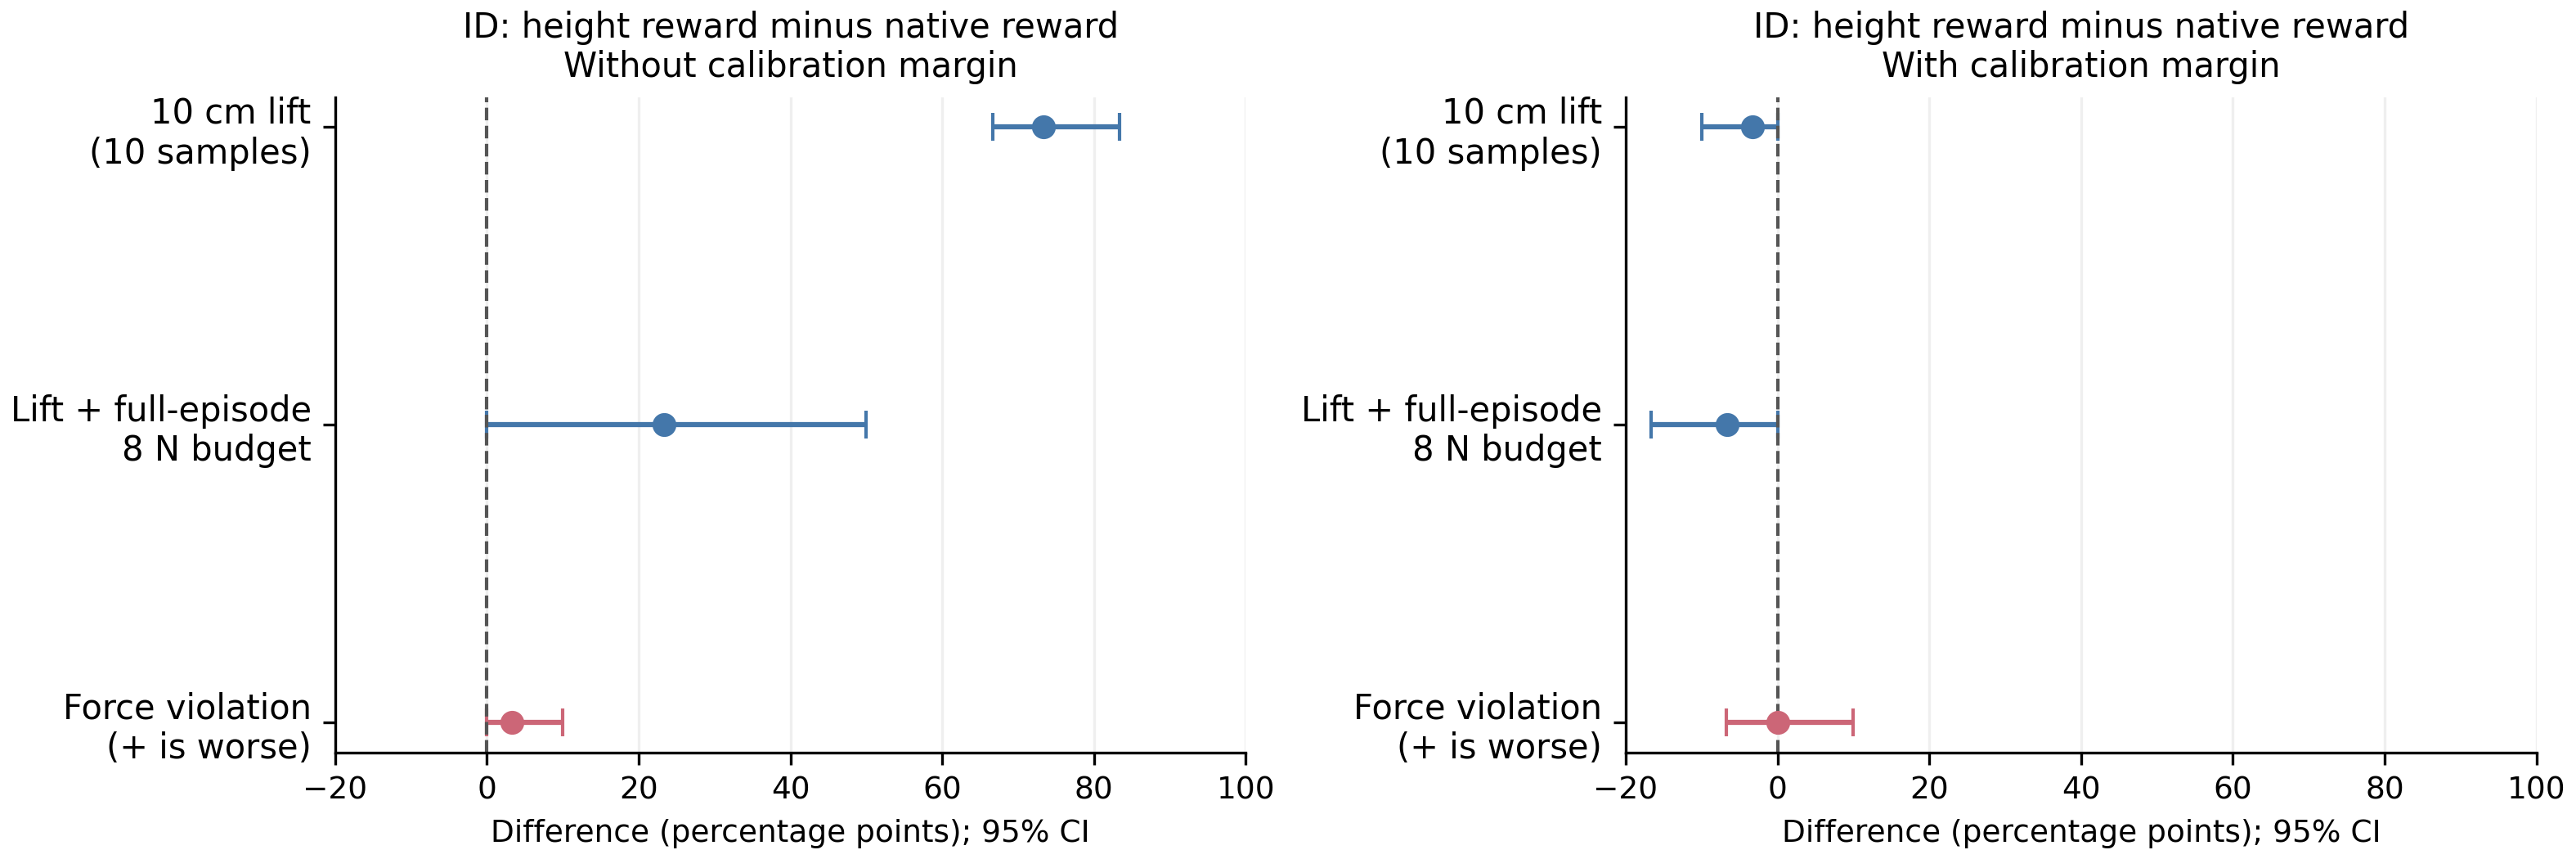
\includegraphics[width=\textwidth]{reward_alignment_id.png}
\caption{Paired second-round ID changes from native to height reward. Intervals
resample the ten shared ID environments while holding the three trained policies
fixed. Better strict lifting does not imply better force regulation.}
\label{fig:reward-alignment}
\end{figure*}

\subsection{Exploratory matched reward revision}

After inspecting the first round, we replace only the imagined task-reward term with $\widehat r_k=\mathrm{clip}(\widehat h_k/0.10,0,1)$, where height is measured in meters. It rewards progress toward the evaluated height at every imagined step, but does not explicitly enforce the ten-observation criterion. Peak penalties, calibration allowances, action ranges, and training settings stay fixed. Audited checkpoint hashes match the original world models, and all six new actors have exactly the same BC initial parameters as their corresponding native-reward actors; the maximum parameter difference is zero. The comparison therefore changes the task-reward term while matching model and actor initialization.

The second round uses twenty fresh environment seeds, 20291000--20291019, again ten ID and ten OOD. The two baselines, three existing visuotactile BC policies, six existing native-reward policies, and six new height-reward policies all execute on this same set. Native policies are re-evaluated here so the reward comparison never mixes the two test cohorts. This follow-up was motivated by observed first-round failures and remains exploratory; its policy matrix was fixed before evaluating the new actors.

Table~\ref{tab:reward-followup} reports the second round; all OOD strict and joint successes remain zero. On ID, height-reward RL achieves strict success counts [9, 10, 9] out of ten for the three seeds, versus [2, 4, 0] for the matched native-reward policies. The paired mean increase is 73.3 percentage points (Fig.~\ref{fig:reward-alignment}), with a fixed-policy, environment-bootstrap 95\% interval of [66.7, 83.3]. Joint success increases by 23.3 points, with interval [0.0, 50.0], while mean episode peak increases by 0.432 N, with interval [0.175, 0.711]. These results support a task-attainment improvement in this follow-up, not improved force regulation. Height-reward joint success remains 36.7 points below feedback, with interval [$-$63.3, $-$10.0].

The margin-height variant attains only 13.3\% ID joint success versus 20.0\% for margin-native; it does not resolve the conservative-margin failure. Repeating the retrospective actual-action diagnostic on the second cohort gives ID joint forecast coverage [10\%, 80\%, 80\%] for height RL, [0\%, 60\%, 50\%] for native RL, and [100\%, 100\%, 100\%] for BC. These are different induced state distributions with unchanged calibration, not evidence of online safety or a universally improved predictor.

\subsection{Computation and scope}

Both rounds together comprise 680 simulator executions but only 40 independent test initial conditions. On the local RTX 5090 Laptop GPU, six world-model training runs take 178.17 s in total; the first nine actor-training runs take 215.13 s and the six follow-up runs take 129.45 s, including replay encoding, BC, and imagined updates. These timings exclude simulator data generation, controller execution, and analysis. World-model training starts from random weights, and the follow-up reuses frozen world models rather than collecting new training interactions.

\section{Limitations and Conclusion}

The experiments support local force prediction and a clear benefit from touch relative to vision-only forecasts. They also expose unfavorable shape transfer, a mismatch between frame and trajectory coverage, large episode-level peak allowances, and persistence baselines that outperform learned dynamics on several force metrics. These results prevent us from attributing the modality gain to useful action-conditioned dynamics alone.

Actual simulator execution shows that a matched, exploratory height-reward revision can improve lifting under the ten-observation criterion relative to native-reward imagination. However, it does not outperform simple force feedback on force-budgeted success and increases mean peak force. The calibration-margin penalty lowers violations with poor task completion, and recording-based forecast coverage degrades under learned policies. Better force regulation, stronger dynamics and reactive baselines, more diverse feasible episodes, and fresh confirmatory evaluation remain necessary to test whether these gains extend to reliable force-constrained control.

The study uses one rigid object geometry, simulated contact-force aggregates, and a small number of independent environments. The reward follow-up lacks a vision-only height-reward ablation, so its control improvement cannot be attributed to touch. Public GelSight data supply a separate sensing result, with no demonstrated transfer to the simulator policy. We do not establish real-robot grasp success, identified friction, deformable-object damage limits, or safety under an optimized policy.

\appendix[Implementation and Reproducibility Details]
\label{sec:implementation}

\subsection{Training settings}
The public-force regressor takes $3\times64\times48$ tactile images. Four
$3\times3$ convolutions with stride two and padding one have 24, 48, 96,
and 128 output channels, respectively; each is followed by eight-group
normalization and SiLU. A 128-unit SiLU hidden layer maps the flattened
feature to three force components. Images are rotated to portrait when
needed and resized bilinearly using the released loader's sample mapping.
Inputs are scaled from bytes to $[-1,1]$; targets use training-only force
means and standard deviations. The loss is mean squared standardized force
error. AdamW uses learning rate $10^{-3}$, weight decay $10^{-4}$, and a
cosine schedule reaching $10^{-4}$ over 30 epochs; batch size is 256 and
gradient norm is clipped at 5. Training uses bfloat16 autocasting, seeds
17, 29, and 43, and trajectory split seed 314159. Minimum validation MAE
selects the checkpoint.

The world-model objective is
\begin{equation}
\begin{aligned}
\mathcal L={}&\mathcal L_F+\mathcal L_p+\mathcal L_h
+0.25(\mathcal L_S+\mathcal L_C)\\
&+0.5\mathcal L_r+0.5\mathcal L_I+20\mathcal L_z.
\end{aligned}
\end{equation}
Here $F,p,h,r$ use elementwise-mean Huber losses with transition point one
after target normalization. Support $S$ and contact $C$ use binary
cross-entropy, $I$ uses RGB mean squared error, and $z$ uses mean squared
latent consistency with the target encoder. Supervision includes the
initial decoded state and five future states; latent consistency uses the
five future states only. AdamW uses learning rate $3\times10^{-4}$,
weight decay $10^{-4}$, batch size 64, and gradient-norm clipping at 20.
The target encoder update rate is 0.01. Each of seeds 0, 1, and 2 trains
both modalities for 25 epochs with training stride three and validation
stride five; minimum validation total loss selects the checkpoint.

The actor has two 128-unit hidden layers and 33,282 parameters. Its
training-data action bounds are approximately $[-0.01133,0.43081]$ for
vertical motion and $[-0.2,1.0]$ for gripper rate. Actor--critic updates
use the hyperparameters in Section~\ref{sec:policy} and a target-value update rate
of 0.01. Encoded training starts lie between actions 44 and 130;
five-step rollouts reaching action 135 terminate without bootstrapping.

\subsection{Measurement and statistical units}
Public-force MAE averages absolute errors over the three force components
and all paired frames. Its interval uses 2,000 bootstrap resamples of whole trajectories,
with seed 20260908, and holds trained regressors fixed. Simulator forecast MAE averages over windows,
five horizons, and the appropriate force components. The reported
training-seed standard deviations quantify variation among three fitted
models; they are distinct from environment-bootstrap confidence intervals.

The strict control metric checks ten consecutive sampled heights at or
above 0.10 m before lowering. At 20 Hz their first and last samples are
0.45 s apart; this metric does not test continuous height between samples.
In contrast, force-budget violations use contact forces at every 0.002 s
physics substep. Each reported force is the sum of normal contact forces
on one finger, and the episode peak maximizes over both fingers and all
substeps, including approach and lowering. Force-budgeted success is the
intersection of strict lift success and no budget violation.

The two control cohorts use environment seeds 20281000--20281019 and
20291000--20291019. Bootstrap intervals use 2,000 paired resamples of
whole environments, stratified by domain, with bootstrap seed 90210.
The same environment draw is used for every fixed policy in a comparison.
These intervals quantify test-environment variation conditional on the
trained policies, rather than uncertainty over repeated policy training.

\section*{Data, Code, and Tool Use}
The public tactile dataset is distributed by its original authors as
\texttt{facebook/gelsight-force-estimation} on Hugging Face under CC BY-NC 4.0.
We use the pinned revision specified above; the original recordings are not
redistributed with this article. Experiment code, split manifests, per-seed
metrics, and per-episode control results accompany the source submission as
ancillary material. The compact model adapts TD-MPC2 components at revision
\texttt{e9f5932}, with the original MIT license retained. No pretrained
world-model weights are used. OpenAI Codex assisted with manuscript drafting
and revision, experiment and analysis code, and experiment orchestration.

\begin{thebibliography}{10}

\bibitem{sparsh}
C.~Higuera \emph{et al.}, ``Sparsh: Self-supervised touch representations for
vision-based tactile sensing,'' in \emph{Proc. 8th Conf. Robot Learning
(CoRL 2024)}, Proc. Mach. Learn. Res., vol.~270, pp.~885--915, 2025.
\url{https://proceedings.mlr.press/v270/higuera25a.html}.
Force-data card:
\url{https://huggingface.co/datasets/facebook/gelsight-force-estimation/blob/main/README.md}.

\bibitem{feelanyforce}
A.-H.~Shahidzadeh, G.~Caddeo, K.~Alapati, L.~Natale, C.~Ferm\"uller, and
Y.~Aloimonos, ``FeelAnyForce: Estimating contact force feedback from tactile
sensation for vision-based tactile sensors,'' in \emph{Proc. IEEE Int. Conf.
Robot. Autom. (ICRA)}, 2025.
\url{https://www.prg.cs.umd.edu/FeelAnyForce}.
Preprint: \url{https://arxiv.org/abs/2410.02048}.

\bibitem{vtwm}
C.~Higuera, S.~Arnaud, B.~Boots, M.~Mukadam, F.~R.~Hogan, and F.~Meier,
``Visuo-tactile world models,'' arXiv:2602.06001v1, 2026.
\url{https://arxiv.org/abs/2602.06001v1}.

\bibitem{feelworld}
W.~Ma, C.~Zhang, C.~Xue, Y.~Cai, G.~Yao, S.~Cui, and S.~Wang,
``FeelWorld: Visuo-tactile world model for hierarchical contact prediction
and planning,'' arXiv:2607.24267v1, 2026.
\url{https://arxiv.org/abs/2607.24267v1}.

\bibitem{omnivta}
Y.~Zheng \emph{et al.}, ``OmniVTA: Visuo-tactile world modeling for contact-rich
robotic manipulation,'' arXiv:2603.19201v3, 2026.
\url{https://arxiv.org/abs/2603.19201v3}.

\bibitem{tdmpc2}
N.~Hansen, H.~Su, and X.~Wang, ``TD-MPC2: Scalable, robust world models for
continuous control,'' in \emph{Proc. Int. Conf. Learn. Representations (ICLR)},
2024. \url{https://openreview.net/forum?id=Oxh5CstDJU}.
Official code: \url{https://github.com/nicklashansen/tdmpc2}.

\bibitem{conformal}
A.~N.~Angelopoulos and S.~Bates, ``Conformal prediction: A gentle introduction,''
\emph{Found. Trends Mach. Learn.}, vol.~16, no.~4, pp.~494--591, 2023.
doi: 10.1561/2200000101.
\url{https://www.nowpublishers.com/article/Details/MAL-101}.

\bibitem{cdt}
J.~Lekeufack, A.~N.~Angelopoulos, A.~Bajcsy, M.~I.~Jordan, and J.~Malik,
``Conformal decision theory: Safe autonomous decisions from imperfect
predictions,'' in \emph{Proc. IEEE Int. Conf. Robot. Autom. (ICRA)}, 2024.
doi: 10.1109/ICRA57147.2024.10610041.
\url{https://arxiv.org/abs/2310.05921v3}.

\bibitem{robosuite}
Y.~Zhu, J.~Wong, A.~Mandlekar, R.~Mart\'in-Mart\'in, A.~Joshi,
K.~Lin, A.~Maddukuri, S.~Nasiriany, and Y.~Zhu,
``robosuite: A modular simulation framework and benchmark for robot learning,''
arXiv:2009.12293v3, 2025. Original preprint, 2020.
\url{https://arxiv.org/abs/2009.12293v3}.

\bibitem{mujoco}
E.~Todorov, T.~Erez, and Y.~Tassa, ``MuJoCo: A physics engine for model-based
control,'' in \emph{Proc. IEEE/RSJ Int. Conf. Intell. Robots Syst. (IROS)},
2012. doi: 10.1109/IROS.2012.6386109.
\url{https://roboti.us/lab/papers/TodorovIROS12.pdf}.

\end{thebibliography}
\end{document}
